\documentclass[man]{apa2}
\usepackage{pslatex}
\usepackage{amssymb}
\usepackage{graphicx}
\usepackage{color}
\usepackage{covington}
\usepackage[usenames,dvipsnames]{xcolor}

\title{Pragmatic contrast helps preschoolers learn category structure\\
Pragmatic inferences as a route to learning category structure\\
Knowledge transmission through pragmatic inference}

\twoauthors{Alexandra C. Horowitz}{Michael C. Frank}
\twoaffiliations{Department of Psychology, Stanford University}{Department of Psychology, Stanford University}


\abstract{Children learn many instances of cultural norms through direct instruction (e.g. ``red lights mean stop''), but not all conventional knowledge is stated explicitly.  We investigate the hypothesis that children infer generalizable information about the world using speakers' descriptive word choices.  We introduced preschoolers to picture triads: an exemplar of a novel category as the base, and then two options that varied from it either by size or by a discrete feature. We described the exemplar using either a size or feature adjective (e.g., ``this is a broken tibu''), and asked children which of the two pictures they thought other category members looked like.  In Experiment 1, we used a supportive framing that signaled that the description was contrastive and found that children reliably made contrast inferences for both size and feature terms.  In Experiment 2, performance was reduced when the contrastive framing was removed and children had to infer contrast from the presence of the adjective alone.  In Experiment 3, we read children a book that highlighted opposite pairs before the task, and this exposure moderately boosted their performance. Preschoolers thus can learn about a novel category from a single exemplar---and not just about what that category is, but also what it isn't. More generally, sensitivity to why speakers choose to describe the world the way they do may allow children to learn efficiently about the world around them. 

~\\

Keywords: pragmatics; language development; adjectives; contrast}

\shorttitle{Learning through pragmatics}
\rightheader{Learning through pragmatics}

\acknowledgements{Special thanks to the staff and families at the Bing Nursery School and the Children's Discovery Museum of San Jose. This work supported by a John Merck Scholars Fellowship and ONR grant N00014-13-1-0287. Earlier versions of this work were presented to the Cognitive Science Society in \citeA{horowitz2012} and \citeA{horowitz2014}.

~\\

\noindent Address all correspondence to Alexandra C. Horowitz, Stanford University, Department of Psychology, Jordan Hall, 450 Serra Mall (Bldg. 420), Stanford, CA, 94305. Phone: 650-721-9270. E-mail: \texttt{ahorowit@stanford.edu}}

\begin{document}

\maketitle                            


\section{Introduction}

%Children learn some cultural information through explicit instruction (e.g., ``put the fork on the left of the plate'') and generic statements (``forks go on the left''), but not all norms are stated directly. We investigate the idea that adults and children may learn generalizable knowledge via Gricean pragmatic inferences about why speakers choose a particular way to convey a message. We focus on the case of learning relevant dimensions of category variability based on the descriptions speakers choose. For example, if a parent says, ``that�s a salad fork,'' he is implicitly revealing that forks vary in the foods they are intended for (and that most other forks are likely used for non-salad items). 


%Many instances of cultural knowledge are taught explicitly.  For example, children are instructed that it is polite to ask for something by saying ``please'' and to receive something by saying ``thank you.''  Some norms, however, are less overtly conveyed and must be inferred through people�s language and actions.  Children may not be told that ``pillows can vary by shape,'' or ``adults like to start the day with coffee,�� yet they nonetheless pick up on this information.  How do children acquire unstated cultural knowledge?  

Children learn some cultural information through explicit instruction (e.g., ``put the fork on the left of the plate'') and generic statements (``forks go on the left''), but not all norms are stated directly. We investigate the idea that adults and children may learn generalizable knowledge via Gricean pragmatic inferences about why speakers choose a particular way to convey a message. We focus on the case of learning relevant dimensions of category variability based on the descriptions speakers choose. For example, if a parent says, ``that�s a salad fork,'' he is implicitly revealing that forks vary in the foods they are intended for (and that most other forks are likely used for non-salad items). Contrastive word choices�particularly (but not limited to) adjectives�can help identify the speaker�s intended referent in the current context (selecting the desired fork) and can jointly signal generalizable knowledge (forks are associated with meal courses). How do children recognize opportunities for inferring cultural conventions?  

Our work investigates one possible hypothesis: Children make inferences about adults� actions (linguistic and non-linguistic) and work backwards to infer the perceived norm or state of the world that motivates these actions \cite{shafto2012}. We test this hypothesis using a simple case study: learning to generalize novel words via the contrastive descriptions that speakers use.  In this paper, we will the development of Gricean pragmatic reasoning as well as children�s inferences about pedagogy and social norms.  We will then describe our three experiments investigating preschoolers' generalizations about unseen category members based on speakers� word choices. 

From the time children begin to speak, they demonstrate some understanding about how language is used to communicate.  Stemming from Grices's maxims (be clear, concise, relevant, and truthful) \cite{grice1975}, young children show early evidence of expecting speakers to communicate cooperatively to expand common ground \cite{clark1996}.  They expect speakers of the same language to use conventional names for conventional meanings \cite{clark1987, markman1988, diesendruck2005}, but learn to recognize that individual knowledge such as facts about objects may not be shared \cite{diesendruck2001}.  Early beliefs that speakers will use language in reliable ways helps children identify information more likely to be culturally normative. 

One salient cue to common knowledge is information conveyed generically.  \citeA{gelman2003} examined 2- to 5-year-olds' comprehension of referential framing cues.  They introduced children to a a picture (e.g. two penguins) and asked ``Can birds fly?'' (generic), ``Can these birds fly?'' (non-generic), or ``Can they fly?'' (pragmatic).  All age groups distinguished generic from non-generic statements, and children also made use of pragmatic cues by age 3.  Children�s sensitivity to generic framing leads them to make different assumptions from generic statements (e.g. ``goats can climb trees'') than non-generic statements (e.g. ``this goat can climb trees��). They are more likely to believe that information stated generically is  conceptually and functionally central and more widely-known \cite{cimpian2009, cimpian2010, cimpian2012}, though also recognize that generic statements may allow more room for variability than strong quantifiers (i.e. ``all'') \cite{gelman2002}.  Children�s appreciation for linguistic framing choices suggests that they are sensitive to how and when cultural information is transmitted.  They pick up on when speakers provide cues to generalizable, conventional information versus more narrow or individualized references. 

%Children also show sensitivity to specific speech decisions speakers make.  From age 3, children can make ad hoc implicatures about a speaker's intended referent (that ``my friend has glasses'' distinguishes a friend with only glasses from a friend with glasses and a hat) \cite{stiller}, 

Children also make inferences about cultural norms and expectations in pedagogical contexts.  Although some evidence indicates that children can make inferences about normative behaviors based on adults� intentional actions alone as an indicator of conventionality \cite{schmidt2011}, stronger cues come from direct labeling.  For example, \citeA{rakoczy2008} introduced 2- and 3-year-old children to a game featuring an action called ``daxing�'' Children then saw a character perform a different action and label it daxing or not.  Both age groups were more likely to protest the new action when it violated their expectations about the meaning of daxing than when it was unlabeled, and by age 3 children were more likely to provide explicitly normative protests (e.g. ``It doesn�t go like that��) than imperative protests (e.g. ``Use the stick''). Providing a label for the action led children to expect and enforce that the action was specific and inflexible to other interpretations.  Even without direct labeling, children expect pedagogical demonstrations to convey complete information: children given a new toy and told, ``This is my toy. I�m going to show you how my toy works. Watch this!�� and a squeaking action were more likely to only use the toy to perform this function than participants who were shown the same action accidentally (``Huh! Did you see that?��) \cite{bonawitz2011}.  Together, these findings suggest that children appear to privilege pedagogical information as conveying cultural expectations about conventional behaviors. 

In our current work, we investigate preschoolers' ability to infer cultural information from the specific word choices speakers choose to produce.  Children show evidence of understanding that conventions are conveyed in particular ways, and we wanted to examine whether children can work backwards to reason about what knowledge a speaker holds in order to produce a specific utterance.  Considering not just \emph{what} speakers say, but \emph{how} they say it may open the doors to available but otherwise untapped sources of information.  We turn to adjective use for a case study in children�s inferences about the implications of word choices.  Because adjectives are syntactical optional in any given utterance, their inclusion may convey important cues about properties of contrast that are relevant to the speaker.  For example, labeling a novel item as a ``tall blicket'' gives information not only that this item is a tall blicket, but it also suggests that height is a relevant variable property to blickets, and that other blickets may be short.  In this way, a speaker may provide valuable implicit information that children could use to infer about non-present category members in the world.  

Indeed, children show evidence of understanding the contrastive nature of prenominal adjectives in their real-time disambiguation by age 3 \cite{fernald2010}, and in more complex referential communication task by kindergarten \cite{nadig2002}, but the work to date has focused on how adjectives are used in contexts.  We examine a novel question by instead asking how adjective use informs the listener of a speaker�s knowledge about the world.  In other words, can children infer that adjective use conveys not only salient information about a present referent, but also clues in the listener to the likely relevant contrastive properties of non-present category members.  

We designed a simple triad task to investigate preschoolers� inferences about adjective use and category membership.  We introduced children to a novel shape, followed by two similar shapes: one that differed from the first only by size, and the other that differed from the first only by feature.  We described the first shape using either a size or feature adjective, and asked children to generalize what they thought other category members looked like.  If children generalize from the exact language heard, then they should expect other category members to share the same property (i.e. if the first shape is labeled as ``small,'' then they should select that other shapes also look small).  if they generalize from the \emph{property choice} conveyed from the speaker�s adjective use, then they should instead select the property \emph{contrast} (i.e. hear ``small'' and select the shape that's bigger).  In Experiment 1, we found that preschoolers' contrast inferences increased from ages 3 --5 years, and were reliably above chance for both size and feature terms by 3.5.  In Experiment 2, performance decreased in a more stripped down version of the task with reduced contrastive framing.  Increased exposure to contrasts after reading a book of opposites before the task moderately recovered performance. 

%Children�s presumptions about labeling conventions extend 

%gricean and pedagogy -- would have said other functions if there were any 

%\cite{schmidt2012}

%A large body of cultural knowledge is never taught�or even described�it is simply presupposed by the way adults talk and act. How do children acquire such knowledge? Our work investigates one possible hypothesis: Children make inferences about adults� actions (linguistic and non-linguistic) and work backwards to infer the perceived norm or state of the world that motivates these actions \cite{shafto2012}. We test this hypothesis using a simple case study: learning to generalize novel words via the contrastive descriptions that speakers use. 

%Our work connects mechanisms of pragmatic inference, which have been well-studied in language development, with processes of cultural learning and generalization. We show that children can figure out that naming a �tall glorp� implies that most glorps are shorter. The same mechanism might also allow them to infer (usefully) that the term �cognitive scientist� implies the existence of other types of scientists, or to infer (negatively) that �female scientist� implies that most scientists�at least in the mind of the speaker�are not female. Thus, pragmatic inferences of the type we study here may constitute an important mechanism of transmission for cultural knowledge. 

%From early word learning, children may use the principle of contrast -- that a contract in form conveys a contrast in meaning \cite{clark1987} -- to infer that modified nouns phrases convey different information than that of bare nouns.  

\section{Experiment 1}

We wanted to investigate whether preschoolers are sensitive to information about the world that is pragmatically conveyed through speakers' word choices. We first investigated preschoolers' sensitivity to implied contrasts using familiar scalar properties.  We reasoned that children may be more likely to infer contrast information when they are able to recognize that the adjective used is a member of an opposite pair (e.g. tall--short). We designed a task in which the choice of adjective was the only informative cue to implicit referential contrast.  If children use adjective information to generalize, they should identify other category members by matching this property.  If they use adjective information to make inferences about implied contrasts, they should identify other category members by whether they contrast along the stated dimension.  We found that young 3--year--olds were unable to systematically recognize category membership through speakers' adjective choices, but age 3.5, children showed sensitivity to implicit dimensions of contrast contained in word choice.  By age 5, children made contrast inferences at similar rates to adults. 



\subsection{Methods}

\subsubsection{Participants}

We recruited a planned sample of 96 children into four age groups: 3.0--3.5 years (n=24, mean age 3;3), 3.5--4.0 years (n=24, mean age 3;9), 4.0--4.5 years (n=24, mean age 4;3), and 4.5--5.0 years (n=24, mean age 4;8).  About half of the sample was recruited from the Bing Nursery School at Stanford University (n=52) and half was recruited from the San Jose Children's Discovery Museum (n=44), divided approximately evenly across age groups.\footnote{Some variability in age and gender counts across locations arises from our commitment to recruit inclusively at the Children's Discovery Museum.  In our partnership, we invite any interested visitors to participate in our studies rather than prescreening children to meet our language requirements or counterbalance all demographic factors \cite{callanan2012}.}


%\foonote{Some variability in age and gender counts across locations arises from our commitment to recruit inclusively at the Children�s Discovery Museum.  In our partnership,  we invite any interested visitors to participate in our studies rather than prescreening children to meet our language requirements }


At the Children's Discovery Museum, parents were asked to fill out a short demographic form about their children's language background.  Only children who were reported to hear English at least 75\% of the time were included in the final sample.  [FILL IN NUMBER] were excluded from analysis based on this criterion\footnote{Bing Nursery School is an English language preschool, and children included in the sample were fluent speakers of English. Children from Bing Nursery School and the Children's Discovery Museum are roughly equated demographically in terms of language exposure, ethnic backgrounds, and parental education, as reported by parents from each location.  Both locations were mainly composed of educated middle class families.  We tested for effect of location, and found no differences across children tested at either location.}.  Children recruited from the museum received a sticker and a certificate for their participation.  An additional [FILL IN NUMBER] were excluded for not completing all four experimental trials, and [FILL IN NUMBER] were dropped from analysis due to interference from parents or siblings interrupting the study procedure. 

[ADD IN GENDER INFO] [ADD IN OTHER MUSEUM DEMOGRAPHIC INFO?]

We also ran a comparison group of 128 adult participants through Amazon's Mechanical Turk online crowd-sourcing service.  Participants were all reportedly native English speakers and residents of the United States.  They were informed that the task was designed for children.  Three participants were excluded for failing to complete the task.  

\subsubsection{Materials}

Children were read a storybook with colorful clipart images.  Each child participated in two training trials and four test trials.  Training trials featured three pictures of familiar items, only two of which shared a contrast property (e.g. chocolate milk, plain milk, and orange juice).  For the test trials, children were shown sets of three similar images: a novel exemplar shape followed by one picture that differed from the exemplar only by size, and one picture that differed from the exemplar only by a feature contrast (e.g. broken versus unbroken) (See Figure \ref{fig:inanimate_demo}). The named size contrasts were \emph{small} (vs. big), \emph{long} (vs. short), \emph{tall} (vs. short), and \emph{short} (vs. long).  The named feature contrasts were \emph{broken} (vs. unbroken), \emph{pointy} (vs. smooth), \emph{dirty} (vs. clean), and \emph{wet} (vs. dry).  To ensure that children were familiar with the contrasts used, a posttest of pictures exemplifying each of these properties was included in a posttest.  Children were able to recognize the contrasts used in our task, with average accuracy of 90\% for 3--3.5 year--olds, 95\% for 3.5--4.0 year--olds, 96\% for 4.0--4.5 year--olds, and 98\% for 4.5--5.0 year--olds.  

The task was adapted to an online format for adults.  Adults viewed a single trial composed of a picture triad and written expressions (see Figure \ref{fig:inanimate_demo}). 

\begin{figure} 
  \begin{center} 
    % 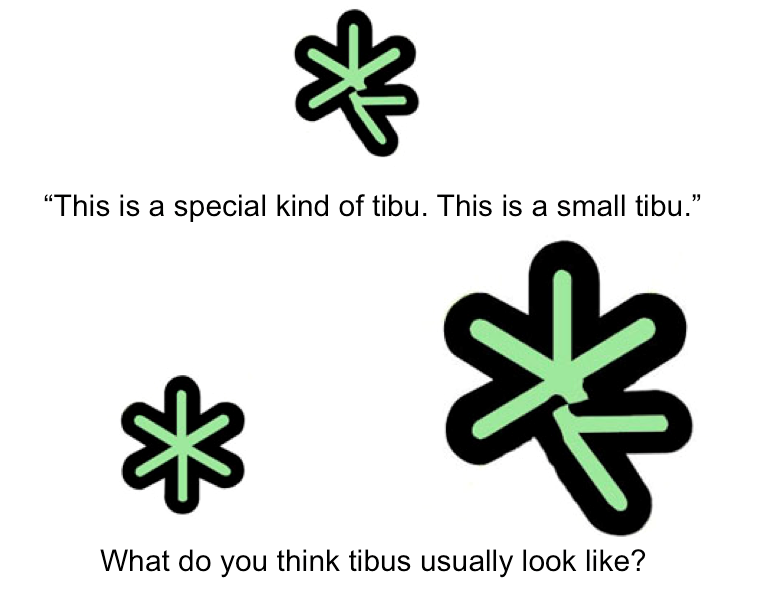
\includegraphics[width=4in]{figures/inanimate_demo.png} 
    \caption{\label{fig:inanimate_demo} Example of a test trial for Experiment 1a.  Children were introduced to an exemplar shaped described with either a size or feature adjective.  They were then shown two images, one that differed from the exemplar by size an done that differed from the exemplar by a feature and were asked to point to which picture they thought was also a member of the same category. } 
  \end{center} 
\end{figure}	



\subsubsection{Procedure}

The experimenter read the storybook with children individually in a quiet room at either Bing Nursery School of the San Jose Children's Discovery Museum.  At the museum, parents accompanied children and sat either next to or behind the child.  Siblings were sometimes also present, and were offered quiet activities such as coloring or reading. 

To begin the book, children were introduced to a character named Allen the Alien who was visiting planet Earth.  Children then participated in two training trials containing familiar items to teach Allen about some things on Earth and get children used to the study design.  Training trials featured adjectives other than those used in critical trials, and training pictures displayed only one relevant contrast choice.  For example, children were shown a picture of chocolate milk followed by two pictures, one of plain milk and one of orange juice.  Children were told, ``This is a special kind of milk.  This is \emph{chocolate} milk.  What does milk usually look like?  What does most milk look like?" and prompted to point to the picture.  On the rare occasion that children answered incorrectly, the experimenter repeated the statements and encouraged children to point to the correct picture until they answered correctly.  

After the training trials, children participated in four test trials.  For each test trial, children were shown a picture of a single exemplar (e.g. a small broken tibu, see Figure \ref{fig:inanimate_demo}) and told something about it, e.g. ``This is a special kind of tibu.  This is a small tibu."  They were then shown two similar pictures, one that differed from the exemplar only by size (i.e. a big broken tibu) and one that differed from the exemplar only by a feature (i.e. a small fixed tibu), and were asked ``What do you think tibus usually look like?  What do you think most tibus look like?".  They were prompted to select one of non-exemplar images.  Two of the four trials used size adjectives (e.g. ``This is a small tibus") and two of the trials used feature adjectives (e.g. ``This is a broken tibu"). The order of trial items varied across two lists, each of which was counterbalanced for adjective type and picture order.  Adjectives were focused using contrastive stress.  The experimenter averted her gaze while children pointed to their responses.  Responses were coded online and double-coded offline using a video recording of the testing session.  The task took about ten minutes to complete. 

Adults were randomly assigned to a single test trial.  Picture type, side, and adjective were counterbalanced across participants.  Adults indicated their response using a radio button below their image selection.  Participants were paid 25 cents for completing the task, which took about two minutes to complete. 

\subsection{Results and discussion}

%Responses were coded as correct if participants selected the shape that differed along the referenced dimension.  In other words, we considered a response to be a correct contrast judgement if the participant selected the shape that differed by feature in feature adjective trials (e.g. heard ``broken'' and selected the shape that was unbroken), and differed by size in size adjective trials (e.g. heard ``small'' and selected the shape that was big).  


We categorized a response as a correct contrast inference if children selected the item that differed from the exemplar along the referenced dimension (i.e. they chose the short item if the exemplar was referred to as ``tall", but the clean item if it was referenced as ``dirty").  We found that preschoolers' sensitivity to contrast information implicit to adjective choice increased from ages 3--6 years of age.  The youngest children in our sample did not demonstrate systematic inferences to adjective information; 3--3.5 year--olds selected the adjective match and the adjective contrast at chance levels when selecting another example of a category member with the referent.  However, by age 3.5, children predictively selected the contrasting property to the adjective named.  Within the early preschool years, children appear to gain sensitivity in assessing speakers' word choice information and the implicit contrast information it may contain. 

Overall, we see that, although even the youngest children in our sample were familiar with the adjectives and their contrast alternatives used in our task, children younger than age 3--and--a--half were unable to reliably use adjective information to infer implicit contrast information.  However, children ages 3.5--4.0 were reliably above chance in selecting the contrast property when size terms were used, and marginally above chance when feature contrasts were used.  Children ages 4.0--4.5 and 4.5--5.0 were reliably above chance in selecting the property contrast across both feature and size terms.  

We analyzed our results using a logistic mixed model, predicting correct responses as an interaction between age and contrast type with random effects of participant and shape.  Children increasingly made more correct contrast judgments with age ($\beta = 1.51$, $p < .0001$).
% There was a significant effect of age, such that children increasingly made more correct contrast judgments with age ($\beta = 1.51$, $p < .0001$).   
  There was no significant effect of contrast type (feature vs. size adjectives), and there was no interaction between age and contrast type, suggesting that participants across ages did not differ in their responses to different property types.  Overall, these analyses show that children demonstrate an increasing sensitivity to implicit contrast information from adjectives.  

Our results indicate that preschoolers are gaining sensitivity to the implications of word choice from ages 3--5 years; by age 4, children were reliably able to use adjective information to infer implied contrasts informing category membership.  We next wanted to determine whether children recognize the informativeness of adjective use across additional, non--scalar properties.  By extending our design to other adjective types, we could examine whether children's early success is due to familiarity with the scalar contrasts used, or whether children assume contrast information from adjective use more generally.  

Participants selected the contrasting dimension more often than chance and at nearly identical rates for both adjective types ($p < .001$ in exact binomial tests for feature and size terms; see Figure \ref{fig:adults_plot}).  Our results indicate that participants used the adjective referenced to make inferences about properties of novel category members, suggesting that adjectives are informative indicators of relevant property information to adults.  They were able to consider the labeled property in order to infer that other novel category members are likely to differ along the referenced dimension. 

Adults had no difficulty making contrast inferences for either the scalar or non-scalar terms.  It appears that children's difficulty inferring implied contrasts from color terms may arise from a lack of experience considering how and why color terms are used. 


\begin{figure}[t] 
  \begin{center} 
    % 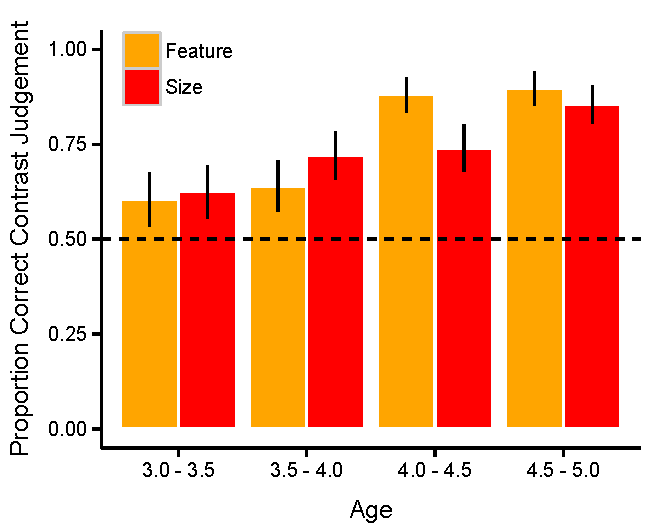
\includegraphics[width=3.5in]{figures/inanimate.pdf} 
    \caption{\label{fig:inanimate} Preschoolers' mean proportion correct performance in Experiment 1b. Yellow bars depict feature adjective trials and red bars depict size trials. The dashed line represents chance (0.5). Error bars represent standard error.}
    %95\% confidence intervals.} 
  \end{center} 
  % \vspace{-2.0ex} 
\end{figure}	


%Participants read a story online in which a cartoon character, Allen the Alien, introduced them to a novel shape from outer space and said something about it, e.g. ``This is a special kind of tibu.  This is a [broken] tibu.'' Half of participants were presented with a feature adjective (e.g. ``broken'') and half were presented with a size adjective (e.g. ``small'').  They were then shown the two test shapes and asked, ``What do you think [tibus] usually look like?'', and prompted to select one of the two images.  We measured the proportion of participants who selected the picture that contrasted with the named property. 


\section{Experiment 2}

In our first set of experiments, we found that adults consistently made contrast inferences from adjective use, while preschoolers gained sensitivity to how speakers mark relevant property information with age.  They may begin by appreciating that scalar opposites are paired, and that use of one term (e.g. \emph{wet}) implies contrast with its opposite (i.e. \emph{dry}). We next wanted to investigate the robustness of children's contrast inferences for opposite terms.  In our first experiments, we tried to make the cues to contrast as strong as possible by conveying contrastive language in our carrier phrase.  In Experiment 2, we eliminated all cues to contrast except for the adjective used: instead of hearing ``This is a special kind of tibu. This is a [small] tibu,'' children instead heard the stripped down expression ``This is a tibu. This is a small tibu.'' This change allowed us to examine children's sensitivity implied contrast from scalar terms without the the support of other pragmatic cues.  We also collected comparison data from a group of adults. 

\subsection{Methods}

\subsubsection{Participants}
A new sample of 48 children was recruited from Bing Nursery School.  Because of the presumed increased difficulty of this task, we recruited children from the older age groups: 4.0--4.5 years (n=24, mean age 4;3) and 4.5---5.0 years (n=24, mean age 4;8). 

We also ran a new group of 128 adult participants on Amazon's Mechanical Turk.  All participants were reported to be US residents and native English speakers.  They were informed that the task was designed for children.  Seven subjects were excluded for failing to complete the task. 

\subsubsection{Materials}
Stimuli were identical to Experiment 1.  

\subsubsection{Procedure}
Procedures were identical to Experiment 1 with the exception that the referential phrase was minimized by removing the phrase ``special kind of'' to reduce contrast cues other than the adjective.  Instead, participants heard only ``This is a [tibu]. This is a [broken tibu],'' isolating the adjective as the only available indicator of category membership.

As in Experiment 1, adults were randomly assigned to a single test trial as seen by children. 

\subsection{Results and discussion}


\begin{figure}[t] 
  \begin{center} 
    % 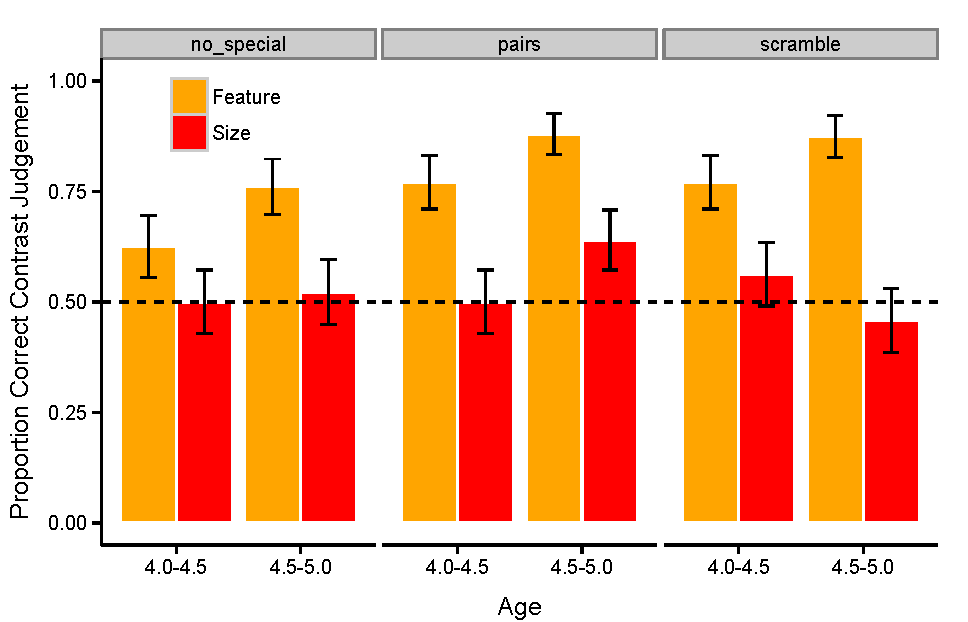
\includegraphics[width=6in]{figures/training_results.pdf} 
    \caption{\label{fig:training_results} Preschoolers' mean proportion correct performance in Experiments 2b and 3.  Feature adjective trials are plotted in yellow and size trials in red. The dashed line represents chance (0.5). Error bars show standard error.}
  \end{center} 
  % \vspace{-2.0ex} 
\end{figure}



	
\begin{figure}[t] 
  \begin{center} 
    % 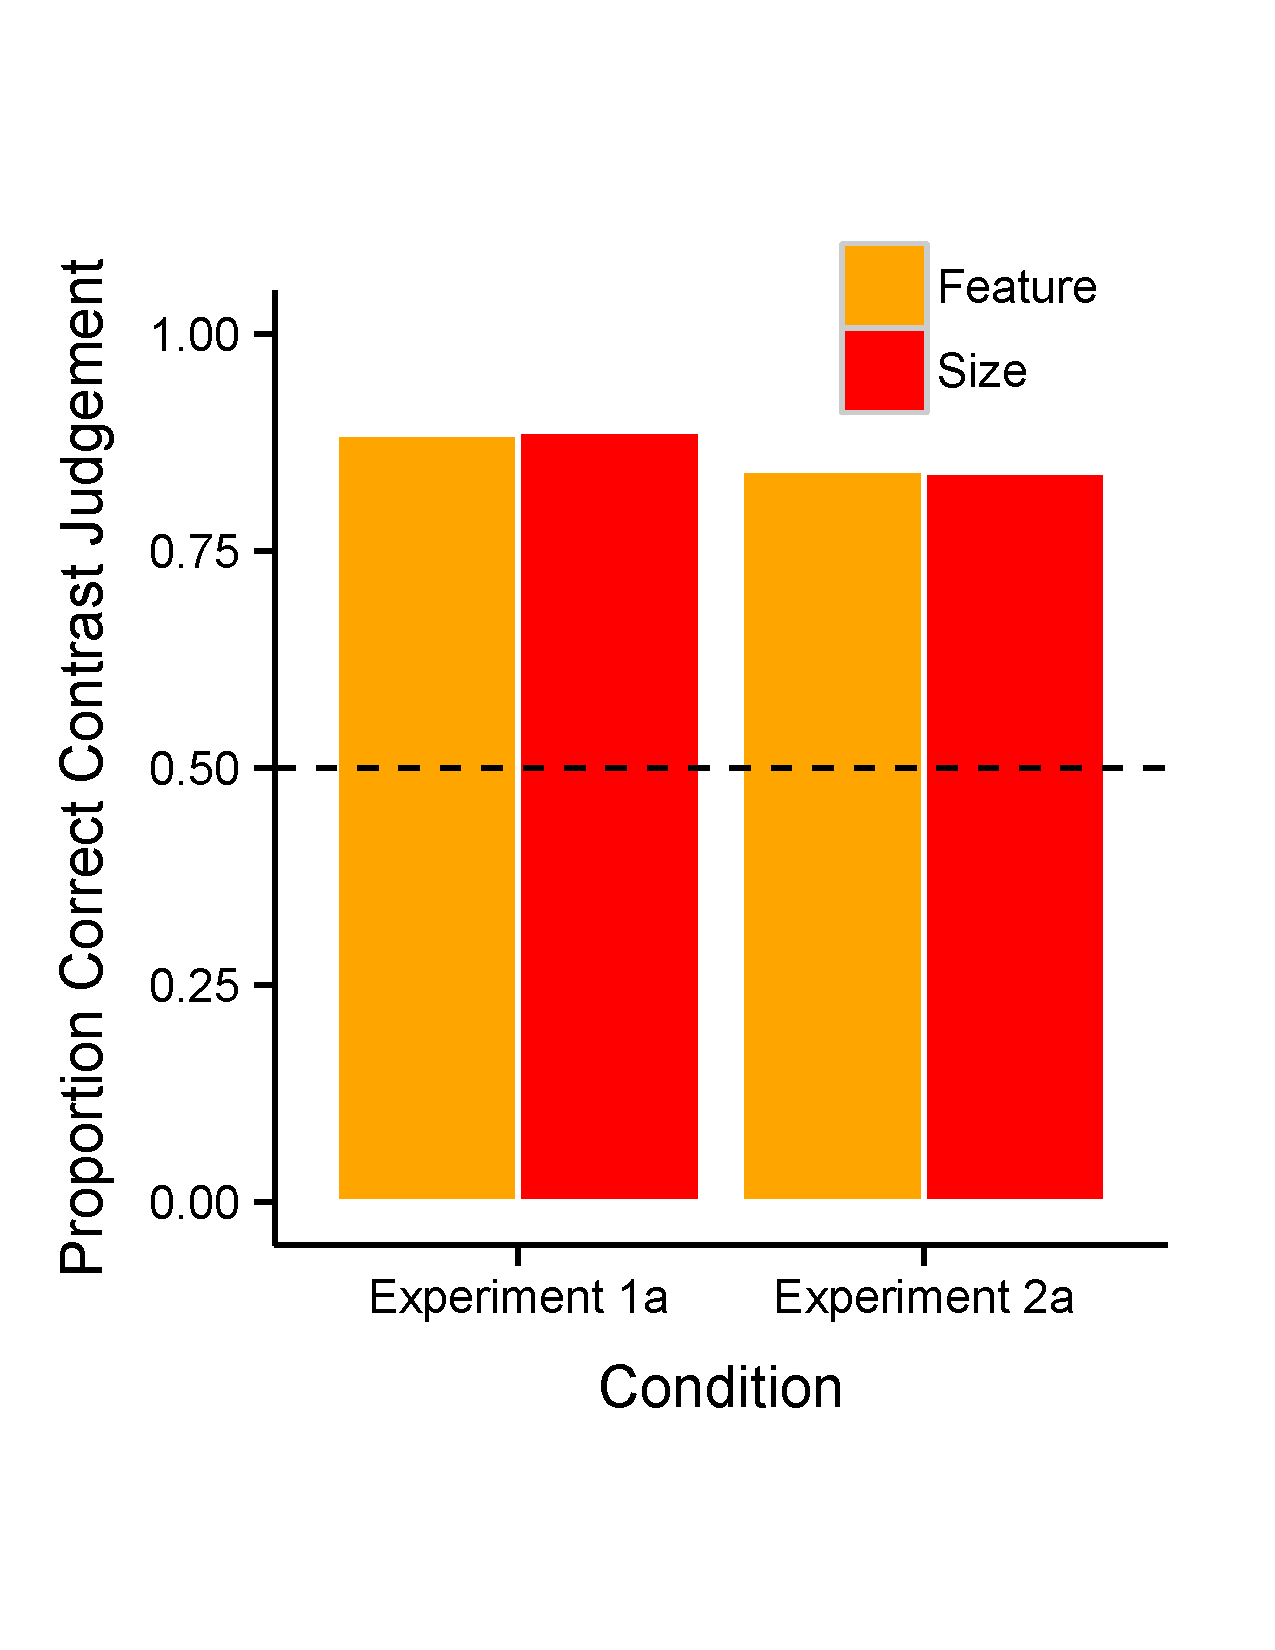
\includegraphics[width=3in]{figures/adults2.pdf} 
    \caption{\label{fig:adults_plot} Adults' mean proportion correct performance in Experiments 1a and 2a. Feature trials are plotted in yellow and size trials in red. The dashed line represents chance (0.5). }
    %Error bars represent 95\% confidence intervals.} 
  \end{center} 
  % \vspace{-2.0ex} 
\end{figure}	


Although preschoolers showed increasing contrast selections from adjective use with age in Experiment 1b, they were essentially at chance when the contrastive language framing was removed.  We analyzed our results using a logistic mixed model, predicting correct responses as an interaction between age and contrast type with random effects of participant and shape, and we found no significant effects and no significant interaction. In post-hoc followup tests, older 4s showed a significant feature contrast bias ($p  = .001$, exact binomial test), but this contrast was not reliable in the full model when controlling for participant and item effects, and may have been driven primarily by the ``broken'' and ``clean'' items. Although adults remained attentive to implicit contrast information in both the contrastive language and adjective only framings, children performed substantially worse without the additional linguistic cues to guide their contrast judgements.  

UPDATE THIS INFO WITH LAST FEW KIDS

As above, we measured the proportion of correct contrast judgments for which participants selected the test picture that differed along the referenced property dimension.  Adults performance was significantly about chance ($p < .001$ in exact binomial tests for feature and size terms) and did not differ by adjective type.  They showed only a slight decrease in performance in this adjective only framing from the contrastive language framing in Experiment 1c (see Figure \ref{fig:adults_plot}).  These results indicate that adjective use in our task is a strong indicator of relevant property information of novel category members for adults.  Their nearly equal performance across Experiment 1a and 2a suggests that adjectives provided salient cues to implicit contrast dimensions on their own without the necessity of additional semantic support. 



\section{Experiment 3} 



%Although children succeeded in forming contrast inferences from adjective with in the contrastive language framing (Experiment 1b), they had difficulty when the adjective was provided on its own without other cues to contrast (Experiment 2b). 

We found a developmental difference in Experiment 2 such that adults robustly made contrast inferences from adjective use alone while preschoolers did not show evidence of reliably picking up on this cue.  We wondered what types of experience might help children gain sensitivity to how and why adjectives are used and what information these word choices convey.  In Experiment 3, we reran Experiment 2 with the modification that we exposed children to the adjectives used at test before undergoing the task.  Children read one of two seemingly unrelated picture books to begin the session: a book that \emph{paired} opposite terms next to each other or a book that contained all the same pages but in a \emph{scrambled} order. If children can recognize that adjectives are used to convey relevant property information after increased familiarity with the mentioned terms, then children in both the \emph{paired} and \emph{scrambled} orders should show a boost in their contrast inferences at test.  If they rely on increased experience that scalar terms imply contrast with specific alternatives, then they should make more contrast inferences after reading the \emph{paired} order book than the \emph{scrambled} order book.  

% If children rely on the support of evidence that adjectives imply contrasts with paired alternatives, then they may gain a boost in their ability to make contrast inferences after being reminded of opposite pairs book.  If they 


%In Experiment 3, we provide a test of the linguistic alternatives hypothesis by increasing preschoolers' access to the relevant lexical alternatives.  Before the experimental procedure, the experimenter read a seemingly unrelated book featuring the opposites referenced in the test trials (see Figure \ref{fig:training_demo}).  This exposure to linguistic alternatives boosted older 4-year-olds' contrast selections. 

\subsection{Methods}

\subsubsection{Participants}

A new planned sample of 48 preschoolers were recruited from Bing Nursery School. Participants were again grouped into two age groups: 4.0--4.5 years (n=24, mean age 4;3) and 4.5--5.0 years(n=24, mean age 4;9).  Half of children within each age group were randomly assigned to the \emph{paired} presentation condition, and the other half were assigned to the \emph{scrambled} presentation condition.  


%4.3225	4.746
%4.238333333	4.764166667
	
%4.280416667	4.755083333
\subsubsection{Materials}

Stimuli were identical to Experiment 2 with the addition of one of two separate training books read prior to the testing procedure.  Each training book consisted of clip art images of familiar items depicting the size and feature contrasts portrayed in the test book. The training books were identical except for the ordering of the pages. In the \emph{paired} condition, opposites were paired so that scalar contrasts were viewed simultaneously and stated consecutively (e.g. ``Here is a small teddybear.  Here is a big teddybear.'')  In the \emph{scrambled} condition, the orders of the pages were mixed up so that consecutive pages conveyed a size and a feature description, and opposites never appeared together (e.g. ``Here is a small teddybear.  Here is a wet car.'') Sample images are presented in Figure \ref{fig:book_demo}.



\begin{figure}[t] 
  \begin{center} 
    % 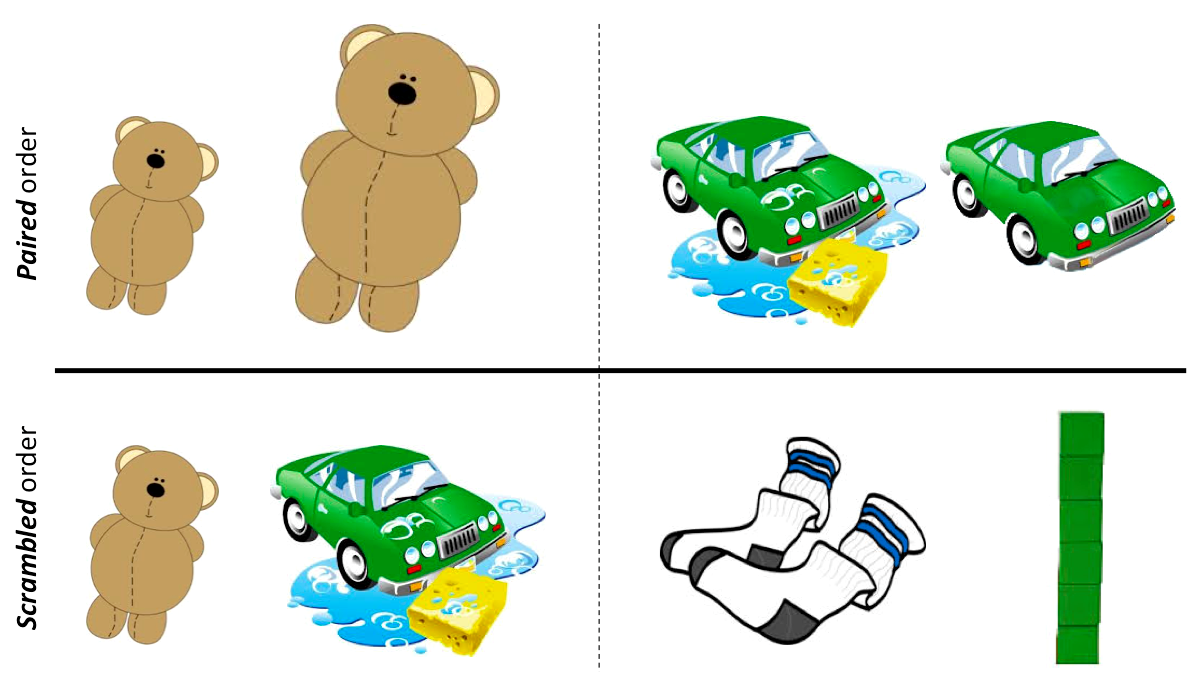
\includegraphics[width=6in]{figures/aliens_book_demo.png} 
    \caption{\label{fig:book_demo} Sample images from the adjectives naming books used in Experiment 3.  The top row depicts two pages of the \emph{paired} condition, in which opposite terms were labeled consecutively (e.g.  ``Here is a small teddybear. Here is a big teddybear.'' and ``Here is a wet car. Here is a dry car.'').  The bottom row depicts two pages of the \emph{scrambled} condition, in which individual opposite terms were interspersed rather than appearing together (e.g. ``Here is a small teddybear. Here is a wet car.'' and ``Here are clean socks. Here is a tall tower of blocks.'').}
  \end{center} 
\end{figure}	




% (e.g. \emph{small/big, broken/fixed}).  Opposite pairs were labeled consecutively to maximize the salience of a given contrast dimension. 

\subsubsection{Procedure}

Children were told that they would be reading two books for the session.  The procedure was identical to that of Experiment 2 with the addition of an adjectives naming book immediately preceding the test book. The experimenter read the adjectives book with children, labeling each picture in a neutral way on each page (e.g. ``Here is a small teddybear. Here is a big teddybear.'').  Children were randomly assigned to read either the \emph{paired} opposites order or the \emph{scrambled} order.  The books were identical except for the order. Although the properties used in adjectives naming books were the same as those in the test book, no child explicitly noted any connection between the books. 

\subsection{Results and discussion}

Increasing preschoolers' access to relevant linguistic alternatives helped older 4s select property contrasts for both feature and size adjectives.  These results suggest that supporting children's abilities to bring relevant alternatives to mind plays a strong role in their pragmatic inferences. Beyond relying on rich semantic framing cues to intended meaning, which are not always available in natural speech, reminding children of different types of modifiers increases their likelihood of forming contrast inferences from adjectives alone. 

Older children selected the contrast property for both feature and size terms more often than chance ($p < .001$ and $p < 0.01$ respectively in exact binomial tests) and younger children for feature terms ($p = .01$ in exact binomial test), though younger children's performance did not differ across feature and size trials.  A logistic mixed model predicting correct responses as an interaction between age and contrast type with random effects of participant and shape revealed no significant effects or interaction, however.

When we combine results with those of Experiment 2b, we find a three-way interaction between experiment, adjective type, and age, such that older children show improved contrast inferences for size terms only after the opposites book ($\beta = 2.60$, $p = 0.04$).  Increased access to lexical alternatives seemed to help older children reliably select the dimension contrast according to the property.  

Our results from Experiment 3 suggest that exposing children to a book of unrelated pictures with the scalar alternatives used in our test trials helped older children to select opposites more consistently, without any framing cues.  An alternative hypothesis, that the initial book served to train children to always select named opposites, is not supported because we did not see a change in performance for the youngest children.  In addition, anecdotally none of the children remarked on any relationship between the books, even though they conveyed the same adjective properties.  Instead, we believe that the opposites book served to make the lexical scales more accessible to children so that, at least for the oldest children in our task, they could spontaneously infer implicit contrast information from an adjective produced alone.   

\section{General Discussion}

Our work connects mechanisms of pragmatic inference, which have been well-studied in language development, with processes of cultural learning and generalization. We show that children can figure out that naming a ``tall glorp'' implies that most glorps are shorter. The same mechanism might also allow them to infer (usefully) that the term ''cognitive scientist'' implies the existence of other types of scientists, or to infer (negatively) that ``female scientist'' implies that most scientists---at least in the mind of the speaker---are not female. Thus, pragmatic inferences of the type we study here may constitute an important mechanism of transmission for cultural knowledge.

\bibliographystyle{apacite2}
\bibliography{ADJ}

\end{document}
